\section{Historia}
% \section{Disclaimer}

% Es por acá, amiga...
% Usuarias de instagram alrededor de Argentina
% creyendo saber por dónde va

A lo largo de la historia, el término \textit{bitácora} ha servido para referir a
distintos objetos relacionados con la orientación, el orden y el registro. Por
primera vez aparecida en un texto escrito en 1538,
%% Fuente: El diccionario etimológico de la lengua castellana de Joan Coromines
la palabra \textit{bitácora}
oficialmente refiere a un concepto de la navegación: \textit{especie de armario
inmediato al timón, en el cual se coloca la brújula}~\cite{dic.Etimologico}.
Desde ahí surge también
el conocido \textit{cuaderno de bitácora}, un libro en el que los marinos, durante
sus guardias, registraban los datos de lo acontecido, y que se guardaba en el
interior de la bitácora para preservarlo de los malos tiempos. El concepto
evolucionó y hoy en día la palabra bitácora usualmente se utiliza para hablar
de registros metodológicos de un suceso particular, ya sea un viaje, una
construcción, etc. Naturalmente, también se transformó la forma en que estos
registros se escriben y dónde se guardan, y existe hoy la noción de \textit{bitácora
virtual}. En esos casos, son las computadoras, las redes y los protocolos,
los que permiten el acceso a esos registros mediante internet; la potencia de la
metáfora garantizando que continúe siendo un concepto de la navegación.
%

En Ciencias de la Computación, las \textit{bitácoras distribuidas} son un tipo de
base de datos que se comparte
alrededor de mútiples lugares, países o instituciones, y que típicamente es de
acceso público. Los registros pueden ser guardados usando distintas estructuras,
y solo pueden agregarse cuando los participantes logran un \textit{quorum}. En
contraste con un sistema centralizado, las bitácoras distribuidas no requieren
un administrador central y, en consecuencia, no tienen un punto de falla central.
Un caso particular de bitácora distribuida, en donde los registros se empaquetan
en forma de bloques, es la \textit{blockchain}.

Las blockchains tomaron
popularidad con la implementación de Bitcoin, una tecnología propuesta por Nakamoto en
2009~\cite{nakamoto06bitcoin}.
Allí se presentó como un método para eliminar terceras partes confiables en sistemas
de pago electrónico.
%

Las versiones más modernas de blockchains incorporan contratos inteligentes~\cite{szabo96smart,ethereum},
los cuales son programas de estado inmutable alojados en la blockchain. Dichos
programas describen la funcionalidad de las transacciones, incluyendo el intercambio
de criptomonedas.
%
Los contratos inteligentes permiten describir funcionalidades sofisticadas, habilitando
diversas aplicaciones en finanzas descentralizadas (DeFi)\footnote{En diciembre de 2021,
el valor monetario alojado en DeFi estaba estimado en alrededor de \$100B, de acuerdo a Statista
\url{https://www.statista.com/statistics/1237821/defi-market-size-value-crypto-locked-usd/}.},
gobierno decentralizado, Web3, etc.
%

Conceptualmente, la blockchain es un \textit{objeto distribuido}
que contiene las transacciones realizadas
en nombre de los usuarios, empaquetadas en bloques, y totalmente
ordenadas~\cite{anta2018formalizing,anta2021principles}.
%
En entornos reales, el objeto blockchain es mantenido por múltiples servidores
sin una autoridad central, usando \emph{algoritmos de consenso} que son resilientes a los
\emph{ataques bizantinos}.
%

%Las blockchains tomaron popularidad
%con la implementación de Bitcoin, un sistema de pago electrónico decentralizado, 
%propuesto por Nakamoto en 2009~\cite{nakamoto06bitcoin}.
%Así, aquello que en sus orígenes fue parte de una herramienta de guía, que mostró
%a los viajeros su rumbo, hoy representa un avance en una dirección que difícilmente se
%pueda considerar certera.

% Agregar alguna cita o reflexión de alguien sobre la humanidad creyendo o queriendo
% conocer el destino

\section{El problema}
% What is the problem. Justifiy that the problem is a problem.

Actualmente, uno de los principales obstáculos para la adopción rápida y generalizada
de las tecnologías blockchain es su límite en la \emph{escalabilidad}, debido principalmente a los límites
de \emph{rendimiento} inerentes a los algoritmos de consenso bizantinos.~\cite{Tyagi@BlockchainScalabilitySol,Croman2016ScalingDecentralizedBlockchain}

En términos generales, la escalabilidad de un sistema es su habilidad para gestionar una
cantidad creciente de trabajo.
%
Usualmente se habla de escalabilidad \emph{horizontal} cuando se añaden nodos de trabajo a un sistema,
en contraposición a la escalabilidad \emph{vertical} que refiere a aumentar los recursos de un nodo particular.

En el caso específico de la tecnología blockchain, la escalabilidad horizontal consiste en añadir nuevos
nodos a la red que participen del protocolo de consenso.
%
Un ejemplo de problema de escalabilidad vertical en este contexto es la creciente cantidad de datos
que requiere almacenar un nodo en la blockchain para guardar transacciones desde el bloque más reciente
hasta el bloque \emph{génesis} (inicial).

En este trabajo nos enfocaremos en la escalabilidad de blockchains desde el punto de vista de su \emph{rendmiento}, medido
en términos del número de transacciones añadidas por segundo.
%
Por dar algunos números representativos de hoy en día, al sistema Bitcoin le toma 10 minutos o más
confirmar transacciones, logrando un rendimiento máximo de 7 transacciones por segundo.
%
Ethereum, una de las blockchains más populares, admite en promedio 20 transacciones por segundo.
%
Estos números son muy bajos comparados con los que observamos en otros campos de pago convencionales,
como PayPal que soporta hasta 200 transacciones por segundo, o Visa, que confirma y procesa 2000 transacciones
por segundo en promedio.
%
Por lo tanto, el rendimiento de las blockchains es un aspecto clave en la adopción de esta tecnología.
%

%  from seven transactions per second to thousands of transactions per second to handle real-life problems in the field of visa, healthcare, flights, etc
% In bitcoin Blockchain 7 transactions are carried out in one
% second ,which is very low compared to VISA and PayPal.
% The time required to confirm the transaction is around 10
% minutes and the size of each block is around 1 MB . 7
% transactions per second is obtained by dividing the
% maximum size of block by an average size of each bitcoin
% transaction as 250 bytes.

% Today’s representative blockchain such as Bitcoin takes 10 min or longer
% to confirm transactions, achieves 7 transactions/sec maximum throughput. In
% comparison, a mainstream payment processor such as Visa credit card confirms a
% transaction within seconds, and processes 2000 transactions/sec on average, with
% a peak rate of 56,000 transactions/sec

% Bitcoin processes 7 transactions per second and Etherium
% processes 20 transactions per second ,whereas payment by
% VISA is 2000 and PayPal is 200 .
% Scaling can be achieved by including more transactions in a
% block .

% Un aspecto clave en la adopción de las tecnologías blockchain es \emph{su rendmiento}, medido
% en términos del número de transacciones añadidas por segundo.
%

\section{Estado del arte}
Diversas técnicas están siendo desarrolladas para incrementar el rendimiento de las blockchains y
aumentar la cantidad de transacciones añadidas por segundo.
%
A continuación se exploran distintas propuestas, intentando abarcar una gama de enfoques novedosos.

\subsection{Desarrollo de algoritmos más rápidos}

En los sistemas blockchains existen múltiples parámaetros que se tienen en cuenta
a la hora de calcular o mejorar el rendimiento de los mismos.
%
En contextos de blockchains que utilizan \emph{proof-of-work}, como Bitcoin, el \emph{ratio de bloque}
se define como el número de bloques minados por segundo.
%
El \emph{tamaño de bloque} se define como el número de bytes en un bloque.
%
Toma tiempo transmitir un bloque sobre la red de pares.
%
El \emph{tiempo de propagación de bloque} se define como el tiempo necesario para que un minero
reciba un nuevo bloque.
%
Dado que un bloque es recibido por diferentes mineros en diferentes momentos, usualmente se utiliza
la \emph{distribución del tiempo de propagación de bloques}.
%
Si se mina un bloque conflictivo mientras otro bloque se propaga en la red, ocurre una bifurcación
(o \emph{fork}) en la red.
%
Los mineros resuelven las bifurcaciones en la blockchain eligiendo la cadena que contiene la mayor
cantidad de bloques.
%
Los bloques no incluidos en la cadena más larga se descartan.
%
El \emph{ratio de bifurcación} se define como el número de bloques descartados por segundo.

Para mejorar el rendimiento de la blockchain no se puede simplemente incrementar el tamaño del bloque
o minar bloques con mayor frecuencia.
%
Hay un triple compromiso entre el tamaño del bloque, el ratio de bloques y el ratio de bifurcación.

FastChain~\cite{fastchain} es un enfoque para mejorar la escalabilidad de los sistemas blockchains
a través de la red de pares.
%
Utiliza un algoritmo de selección del mejor vecino para reducir el tiempo de propagación de los bloques.
%
De esta forma, los mineros se desconectan de los vecinos con ancho de banda limitado y
favorecen a los nodos con mayor ancho de banda.

\begin{figure}
  \centering
  \subfloat[Política aleatoria.]{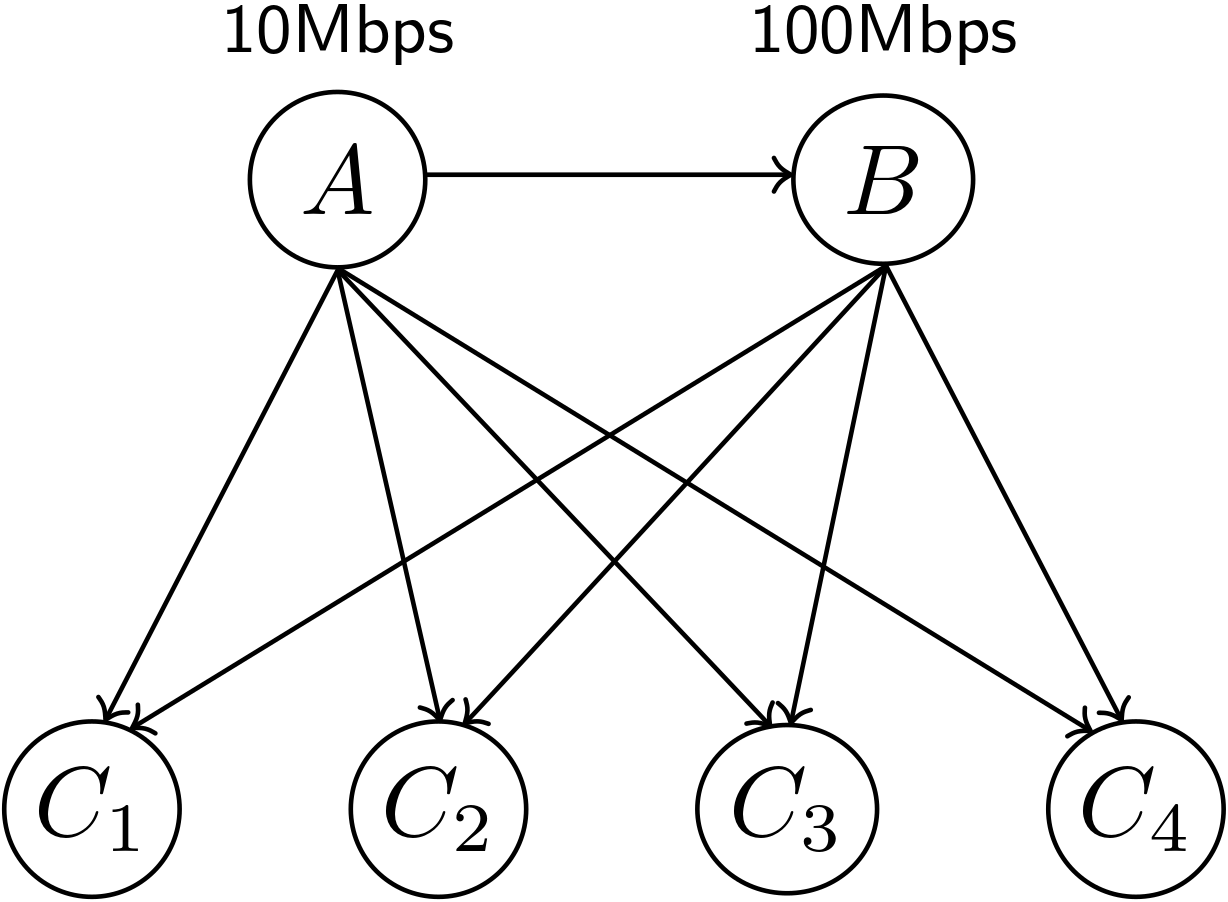
\includegraphics[scale=0.1]{figures/fastchain0.png}\label{subfig:fastchain-a}}
  \hspace{1.5cm}
  \subfloat[Política de FastChain.]{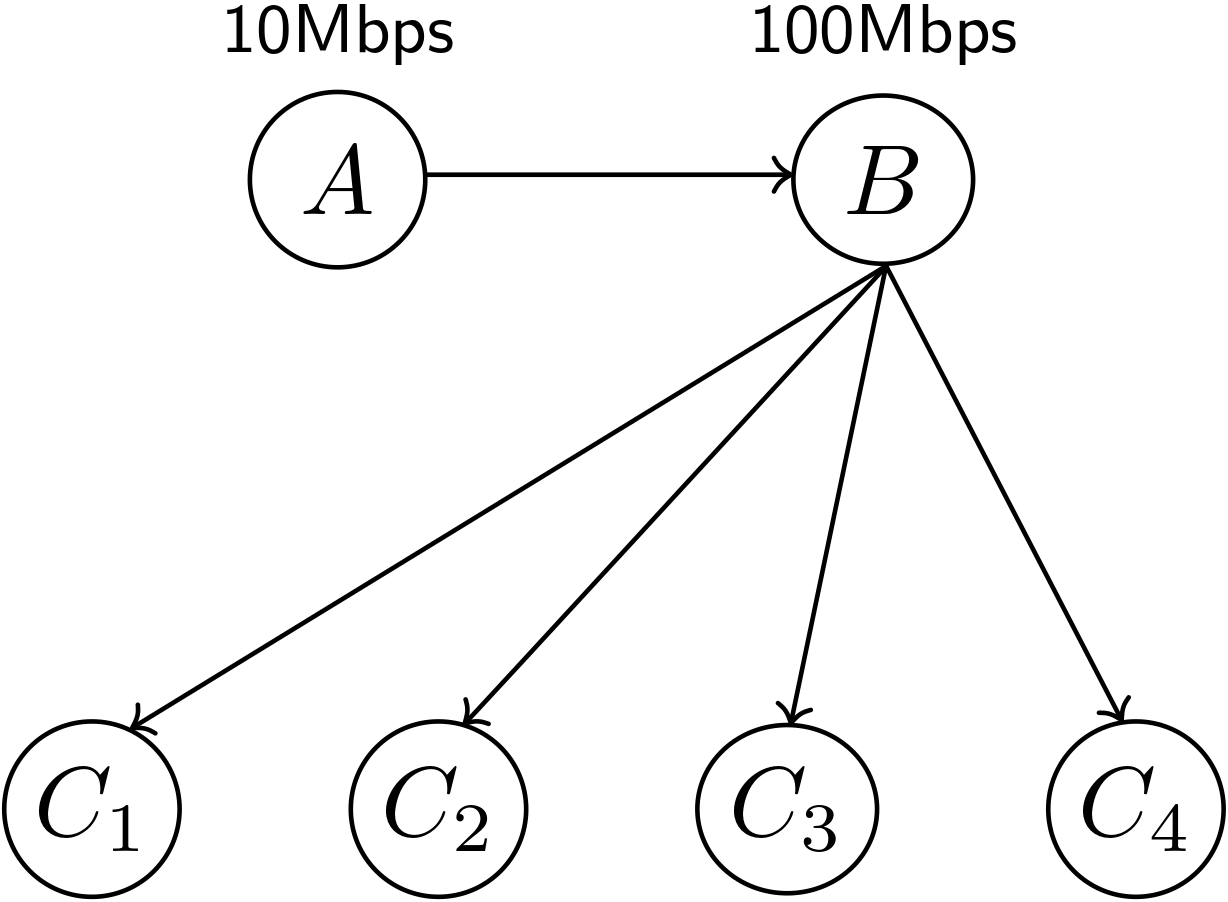
\includegraphics[scale=0.1]{figures/fastchain1.png}\label{subfig:fastchain-b}}
  \caption{Selección de vecinos. Ejemplo motivador para FastChain}
  \label{fig:fastchain}
\end{figure}

En la Figura \ref{fig:fastchain} se muestra un ejemplo motivador para la lógica detrás de FastChain.
%
El nodo $A$ tiene 10Mbps de ancho de banda.
%
El nodo $B$ tiene 100Mbps.
%
Todos los enlaces tienen 200ms de latencia.
%
La Figura \ref{subfig:fastchain-a} corresponde a una política de selección de vecinos aleatoria.
%
Los nodos $A$ y $B$ tienen 5 vecinos.
%
La Figura \ref{subfig:fastchain-b} muestra una política de selección de vecinos
con información de ancho de banda.
%
El nodo $A$ se conecta únicamente con el nodo $B$, mientras que el nodo $B$ se conecta
a todos los otros.
%
Supongamos que el nodo $A$ mina un bloque de tamaño $10^6$ bytes.
%
En la Figura \ref{subfig:fastchain-a}, el ancho de banda del nodo $a$ se reparte entre las 5 conexiones.
%
Cada conección tiene un ancho de banda de 2Mbps.
%
Por lo tanto, a sus vecinos les toma 4.2s recibir el nuevo bloque.
%
En la Figura \ref{subfig:fastchain-b}, el nodo $A$ primero le transmite el bloque a $B$ en 1s.
%
El nodo $B$ luego transmite el bloque al resto de los nodos en 0.52s.
%
El tiempo de propagación de bloque promedio en la topología de FastChain es 1.416s,
casi 3 veces menor que su contraparte para la topología de selección de vecinos aleatoria.
%

El nodo $A$ es el cuello de botella para la propagación de bloques.
%
Mientras el nodo $A$ está transmitiendo el bloque, otros nodos con mayor ancho de banda
están ociosos.
%
FastChain propone una política de selección de vecinos para escalar el sistema blockchain.

\subsection{\emph{Inter-Blockchain Communication}}
La tecnología blockchain está creciendo masivamente; el número de plataformas y
aplicaciones decentralizadas se incrementó rápidamente en los últimos años.
%
Sin embargo, la mayoría de las redes de blockchain operan en entornos autónomos aislados
de los demás.
%
La interoperabilidad de blockchains es la habilidad de conectar mútiples redes de
blockchain entre sí, lo cual puede constituir un enfoque para mejorar la escalabilidad en
las plataformas.
%
De esta forma múltiples blockchains paralelas pueden interoperar, manteniendo las
propiedades de seguridad de las mismas.

Una arquitectura novedosa de redes de blockchains es Cosmos, que conecta diversas
blockchains independientes, llamadas \emph{zonas}.
%
Las zonas funcionan con Tendermint Core, un motor de consenso consistente de alto rendimiento.
%
El algoritmo de consenso del Tendermint Core es adecuado para escalar blockchains públicas que
trabajan con modelos \emph{proof-of-stake}.
%
Sin embargo, blockchains con modelos de consenso \emph{proof-of-work}, como Bitcoin o Ethereum,
se pueden conectar a la red de Cosmos utilizando adaptadores de zonas.

% Blockchain technology is growing massively where the number of
% blockchain platforms and decentralized applications are increasing
% rapidly in the last years. However, most of the existing blockchain
% networks are operating in a standalone environment isolated from
% each other, which increases scalability and connectivity issues in
% the current blockchain platforms as well as limiting the
% blockchain adoption in industry ecosystems. In the current phase,
% different blockchain networks don’t have mutual trust where they
% cannot interact with each other and their capacity level has only
% reached a level similar to LAN. Due to the high barriers between
% the independent isolated blockchain platforms, researchers have
% started to focus on the concept of Blockchain interoperability.
% Blockchain interoperability is the ability of connecting multiple
% blockchain networks together, which significantly increases and
% solves scalability and connectivity issues in the blockchain
% platforms.
% An ideal solution is one that allows multiple parallel blockchains to interoperate while retaining their security properties.

% Here we present Cosmos, a novel blockchain network architecture that addresses all of these problems.
% Cosmos is a network connecting many independent blockchains, called zones. The zones are powered by Tendermint Core [8],
% which provides a high-performance, consistent, secure PBFT-like consensus engine, where strict fork-accountability guarantees
% hold over the behaviour of malicious actors. Tendermint Core's BFT consensus algorithm is well suited for scaling public
% proof-of-stake blockchains. Blockchains with other consensus models, including proof-of-work blockchains like Ethereum and
% Bitcoin can be connected to the Cosmos network using adapter zones.

La primera zona de Cosmos se llama \emph{Cosmos Hub}.
%
Cosmos Hub conecta varias blockchains (o zonas) mediante un protocolo de comunicación entre blockchains,
funcionando como un protocolo TCP para blockchains.
%
Gestiona numerosos tipos de \emph{tokens} y mantiene un registro del número total de los mismos en cada zona conectada.
%
Los tokens pueden transferirse de una zona a otra de forma segura y rápida sin necesidad de un intercambio \emph{líquido} entre zonas.
%
En su lugar, todas las transferencias de tokens inter-blockchains pasan a través del Cosmos Hub.
%
En la Figura se ilustra un ejemplo simplificado de esta arquitectura.

La interaoperabilidad de blockchains ...

[AÑADIR REFERENCIAS] [AÑADIR IMÁGENES]
% Esta arquitectura resuelve muchos problemas a los que se enfrenta actualmente el espacio blockchain, como la interoperabilidad de las aplicaciones,
% escalabilidad y capacidad de actualización sin fisuras. Por ejemplo, las zonas derivadas de Bitcoind, Go-Ethereum, CryptoNote, ZCash, o
% cualquier sistema de cadena de bloques. Estas zonas permiten a Cosmos escalar infinitamente para satisfacer la demanda global de transacciones.
% demanda global de transacciones. Las zonas son también un gran ajuste para un intercambio distribuido, que será apoyado también.

% Cosmos no es sólo un libro mayor distribuido, y el Hub Cosmos no es un jardín amurallado o el centro de su universo.
% Estamos diseñando un protocolo para una red abierta de libros de contabilidad distribuidos que puede servir como una nueva base para
% futuros sistemas financieros,
% basado en principios de criptografía, economía sólida, teoría del consenso, transparencia y responsabilidad.

% A constant stream of recent block commits from zones posted on the Hub allows the Hub to keep up with the state of each zone.
% Likewise, each zone keeps up with the state of the Hub (but zones do not keep up with each other except indirectly through the Hub).
% Packets of information are then communicated from one zone to another by posting Merkle-proofs as evidence that the information was
% sent and received. This mechanism is called inter-blockchain communication, or IBC for short.


\subsection{Paralelismo}
Los sistemas de base de datos tradicionales logran escalabilidad dividiendo
los estados de la base de datos en fragmentos independientes (o particiones).
%
Al distribuir la carga sobre múltiples particiones, la capacidad global del sistema
se incrementa.
%
La técnica de \emph{sharding} requiere cierta coordinación para lograr propiedades
básicas de atomocidad, consistencia, aislamiento y durabilidad para aquellas transacciones
que acceden a múltiples fragmentos.
%
En la Figura se representa la idea de \emph{sharding} como la combinación entre
réplica y partición.
%
Cada partición se replica sobre múltiples réplicas, y su contenido se mantiene consistente
mediante protocolos de consenso.

En el contexto de blockchains, el enfoque de \emph{sharding} se basa en aplicar este concepto
originario de la escalabilidad de bases de datos, dividiendo la red de blockchain en comités más
pequeños de modo de reducir la sobrecarga de los protocolos de consenso.
%
Sin embargo, este concepto no puede ser directamente extendido a los sistemas de blockchain, debido
a diferencias fundamentales en los modelos de fallas que se consideran en las bases de datos
y en las blockchains.
%
Tradicionalmente, las bases de datos asumen modelos de fallo por caída, en los cuales un nodo que falla
simplemente deja de enviar y responder peticiones.
%
Por el otro lado, los sistemas de blockchain operan en ambientes más hostiles, asumiendo modelos de fallas
más fuertes, conocidos como bizantinos, que tienen en cuenta a atacantes malintencionados.
%
La Figura remarca las diferencias entre las bases de datos distribuidas y las blockchains fragmentadas,
mostrando la necesidad de un protocolo de formación de particiones.

[AGREGAR IMÁGENES]
[AGREGAR REFERENCIAS]
% Traditional databases assume the crash-failure model, in which a
% faulty node simply stops sending and responding to requests. On
% the other hand, blockchain systems operate in a more hostile environment, therefore they assume a stronger failure model, namely
% Byzantine failure, to account for malicious attackers. Figure 1 highlights the differences between distributed databases and sharded
% blockchains


% approach is to use sharding, a well-studied and proven
% technique to scale out databases, to divide the blockchain network
% into smaller committees so as to reduce the overhead of consensus
% protocols. Examples of sharded blockchains include Elastico [33],
% OmniLedger [27] and RapidChain [49].

% Two important coordination protocols are distributed commit such as twophase commit (2PC) which ensures atomicity, and concurrency
% control such as two-phase locking (2PL) which achieves isolation.
% In this paper, we use the term sharding to refer to the combination
% of replication and partitioning as shown in Figure 1a.
% This architecture is adopted by recent distributed database systems to achieve
% fault tolerance and scalability [22]. Each partition is replicated over
% multiple replicas, and its content is kept consistent by consensus
% protocols [29, 42]. Transaction management and consensus protocols can be combined more judiciously, as opposed to layering one
% on top of another, to achieve better performance [40, 48, 50].

% Sharding in database systems assumes crash-failure model, in
% which a faulty node stops sending and responding to requests.
% There are three important implications of this assumption. First,
% efficient consensus protocols catered for crash-failure model can
% be used to achieve high performance. Second, creating a shard is
% simple. For example, a node can be assigned to a shard based on its
% location. Third, the coordinators that drive coordination protocols
% are fully trusted

% sharding is a well-studied and proven technique to scale out databases.
% In this work, we take a principled approach to apply
% to blockchain systems in order to improve their transaction throughput at scale.

\subsection{Capa 2}
Los enfoques para incrementar el número de transacciones por segundo en las blockchains pueden
ser categorizados según la \emph{capa} que involucran.
%
Las técnicas de capa 0 son aquellas que trabajan sobre la instraestructura de la red.
%
Por ejemplo, apostando a decrementar la latencia de la misma.
% 
La capa 1 es la que cuenta con más propuestas en la literatura, abarcando todas aquellas que
mejoran los algoritmos de consenso.
%
Por último, la capa 2, también conocida como \emph{off-chain} (fuera de la cadena),
incluye aquellos protocolos que funcionan con una interacción mínima con la
blockchain.

Existen diferentes enfoques dentro de la capa 2.
%
Uno de los principales consiste en la computación \emph{off-chain} de pruebas de \emph{conocimiento cero}
(\emph{Zero-Knowledge proofs}), que solo necesitan ser validadas dentro de la cadena.
%
La adopción de funcionalidades limitadas (pero útiles) de canales es otra técnica perteneciente a la capa 2.
%
Por último, tecnologías conocidas como \emph{optimistic rollups} se basan en evitar ejecutar contratos inteligentes
en los servidores, manteniendo la mínima sincronización requerida con la cadena para preservar las garantías
de la blockchain (por ejemplo, cuando se necesitan anotar reclamos o resolver disputas).

[AGREGAR REFERENCIAS]

\subsection{\setchain}
Las blockchains actuales requieren de algoritmos de consenso que garanticen que las
transacciones, empaquetadas en bloques, estén totalmente ordenadas.
%
Esta imposición de un orden total puede ser innecesaria para algunas aplicaciones.

%
Un enfoque prometedor para escalar la cantidad de transacciones agregadas por segundo
es \textit{Setchain}~\cite{Capretto.2022.Setchain},
un tipo de datos concurrente que implementa conjuntos de solo crecimiento distribuidos,
proveyendo barreras o puntos de sincronización (llamados épocas).
% A su vez, \textit{Setchain} es tolerante a comportamientos bizantinos.
%
\setchain relaja el requerimiento de orden total y, por lo tanto, logra mayor
rendimiento y escalabilidad.
%
Las \setchains se pueden usar para aquellas aplicaciones, como los registros digitales,
en donde los elementos en la blockchain no necesitan estar ordenados, excepto a través
de barreras ocasionales.

%
Distintos algoritmos bizantinos distribuidos que implementan \setchain fueron
propuestos, pero no existía al momento ninguna implementacion eficiente compatible con
los requerimientos de una aplicación del mundo real.
Es decir, una aplicación capaz de soportar un \textit{deployment} con miles de nodos\footnote{Si bien
es difícil saber con exactitud cuántos nodos existen en la red de Blockcahin o Ethereum, se estima
que este número varía entre aproximadamente 10000 y 50000 nodos.}
distribuidos geográficamente en todos los continentes, con clientes enviando peticiones para
añadir nuevas transacciones a los servidores constantemente.

\section{Contribuciones}
En este trabajo se propone una familia de implementaciones robustas de \setchain,
construidas sobre la plataforma de aplicación de blockchain \textit{Tendermint}.

%% Motivate the use of tendermint. Why tendermint is relevant

% Fuente: TENDERMINT: BYZANTINE FAULT TOLERANCE IN THE AGE OF BLOCKCHAINS
% https://docs.tendermint.com/v0.34/introduction/what-is-tendermint.html

Tendermint~\cite{Buchman.2018.Tendermint} es una plataforma novedoza y popular para la
replicación segura y consistente de aplicaciones en distintas máquinas.
%
\textit{Segura} en este contexto significa que Tendermint funciona incluso si a lo sumo
un tercio de las máquinas falla de formas arbitrarias, brindando información conflictiva
a las diferentes partes del sistema.
%
\textit{Consistente} refiere a que toda máquina correcta verá el mismo lote de
transacciones y computará el mismo estado.
%
Tendermint es un abordaje robusto de las blockchains implementado
en \emph{Go}~\cite{donovan15go}, que presenta una separación clara entre las
capas de bajo nivel de la blockchain,
tales como un protocolo \textit{gossip} y un algoritmo de consenso, y los conceptos de alto
nivel relacionados a la estructura de datos que la blockchain mantiene\footnote{Al momento
de la realización de las implementaciones y la evaluación empírica de las mismas,
Tendermint 0.34 era la versión de la plataforma vigente y más utilizada. Sin embargo,
actualmente, la versión más utilizada es un \textit{fork} de Tendermint llamado \textit{CometBFT}~\cite{cometbft.repo}.
El desarrollo planteado a lo largo de este trabajo podría en principio portarse a la nueva versión sin demasiado esfuerzo.}.

%
% What is the solution.
%

La familia de implementaciones que se presenta en este trabajo
sigue un enfoque incremental, proveyendo diversas aproximaciones
a la solución final y más compleja; consta de tres variantes:
\begin{itemize}
  \item \textit{\vanilla}, una primera solución básica de \setchain, en donde cada elemento añadido
  a la \setchain se traduce como una transacción en la blockchain.
  \item \textit{\compresschain}, una variante intermedia que usa un algoritmo de compresión,
  en la cual los elementos enviados por los clientes son agrupados en un lote, que se comprime antes
  de transmitirse como una transacción. Por lo tanto, las transacciones en la blockchain son
  lotes comprimidos de elementos.
  \item \textit{\hashchain}, la contribución principal de este trabajo, una solución 
  a \setchain usando funciones hash. Sigue una lógica similar a \compresschain,
  en donde los elementos se agrupan en lotes y se aplica una función hash antes de transmitirlos
  como una única transacción de tamaño fijo.
\end{itemize}
%
Hashchain explota el poder de compresión de las funciones hash para reducir la
comunicación necesaria durante difusión y consenso, comunicando un hash de tamaño
fijo en lugar de cientos o miles de elementos.
%
El precio a pagar es un algoritmo distribuido adicional para obtener el conjunto de
elementos desde un hash, garantizando tolerancia a servidores bizantinos.
%

La hipótesis fundamental con la que se trabaja es que intercambiar latencia por un aumento en el
ancho de banda resulta en una mejora significativa en el rendimiento.
%
Es decir, hacer consenso sobre hashes de tamaño fijo conlleva un incremento en la cantidad de elementos
añadidos a la \setchain por segundo, incluso si esto significara un aumento en la latencia.

Cada una de las soluciones presentadas en este trabajo está enteramente construida sobre Tendermint.

% The article is structured as follows: in Section~\ref{sec:prelim}, we present a
% brief description of Setchain and Tendermint; in Section~\ref{sec:impl}, we
% describe three implementations of Setchain on top of Tendermint; and in
% Section~\ref{sec:conclusion}, we conclude our work.
% %
% This article is presented as a work-in-progress and shows partial results, and
% thus, the experimental section is lacking.

% We prove how Hashchain can implement Setchain correctly.

%%% Local Variables:
%%% TeX-master: "article.tex"
%%% TeX-PDF-mode: t
%%% End:
